\begin{enumerate}[label=\thesubsection.\arabic*,ref=\thesubsection.\theenumi]
\item Find the shortest distance between the lines
\begin{align}
	\frac{x+1}{7}&=\frac{y+1}{-6}=\frac{z+1}{1} \text{ and}
	\\
	\frac{x-3}{1}&=\frac{y-5}{-2}=\frac{z-7}{1}
\end{align}
    \solution
		\iffalse
\documentclass[journal,12pt,twocolumn]{IEEEtran}
\usepackage{romannum}
\usepackage{float}
\usepackage{setspace}
\usepackage{gensymb}
\singlespacing
\usepackage[cmex10]{amsmath}
\usepackage{amsthm}
\usepackage{mathrsfs}
\usepackage{txfonts}
\usepackage{stfloats}
\usepackage{bm}
\usepackage{cite}
\usepackage{cases}
\usepackage{subfig}
\usepackage{longtable}
\usepackage{multirow}
\usepackage{enumitem}
\usepackage{mathtools}
\usepackage{steinmetz}
\usepackage{tikz}
\usepackage{circuitikz}
\usepackage{verbatim}
\usepackage{tfrupee}
\usepackage[breaklinks=true]{hyperref}
\usepackage{tkz-euclide}
\usetikzlibrary{calc,math}
\usepackage{listings}
    \usepackage{color}                                            %%
    \usepackage{array}                                            %%
    \usepackage{longtable}                                        %%
    \usepackage{calc}                                             %%
    \usepackage{multirow}                                         %%
    \usepackage{hhline}                                           %%
    \usepackage{ifthen}                                           %%
  %optionally (for landscape tables embedded in another document): %%
    \usepackage{lscape}     
\usepackage{multicol}
\usepackage{chngcntr}
\DeclareMathOperator*{\Res}{Res}
\renewcommand\thesection{\arabic{section}}
\renewcommand\thesubsection{\thesection.\arabic{subsection}}
\renewcommand\thesubsubsection{\thesubsection.\arabic{subsubsection}}

\renewcommand\thesectiondis{\arabic{section}}
\renewcommand\thesubsectiondis{\thesectiondis.\arabic{subsection}}
\renewcommand\thesubsubsectiondis{\thesubsectiondis.\arabic{subsubsection}}

% correct bad hyphenation here
\hyphenation{op-tical net-works semi-conduc-tor}
\def\inputGnumericTable{}                                 %%

\lstset{
frame=single, 
breaklines=true,
columns=fullflexible
}

\begin{document}


\newtheorem{theorem}{Theorem}[section]
\newtheorem{problem}{Problem}
\newtheorem{proposition}{Proposition}[section]
\newtheorem{lemma}{Lemma}[section]
\newtheorem{corollary}[theorem]{Corollary}
\newtheorem{example}{Example}[section]
\newtheorem{definition}[problem]{Definition}
\newcommand{\BEQA}{\begin{eqnarray}}
\newcommand{\EEQA}{\end{eqnarray}}
\newcommand{\define}{\stackrel{\triangle}{=}}

\bibliographystyle{IEEEtran}
\providecommand{\mbf}{\mathbf}
\providecommand{\pr}[1]{\ensuremath{\Pr\left(#1\right)}}
\providecommand{\qfunc}[1]{\ensuremath{Q\left(#1\right)}}
\providecommand{\sbrak}[1]{\ensuremath{{}\left[#1\right]}}
\providecommand{\lsbrak}[1]{\ensuremath{{}\left[#1\right.}}
\providecommand{\rsbrak}[1]{\ensuremath{{}\left.#1\right]}}
\providecommand{\brak}[1]{\ensuremath{\left(#1\right)}}
\providecommand{\lbrak}[1]{\ensuremath{\left(#1\right.}}
\providecommand{\rbrak}[1]{\ensuremath{\left.#1\right)}}
\providecommand{\cbrak}[1]{\ensuremath{\left\{#1\right\}}}
\providecommand{\lcbrak}[1]{\ensuremath{\left\{#1\right.}}
\providecommand{\rcbrak}[1]{\ensuremath{\left.#1\right\}}}
\theoremstyle{remark}
\newtheorem{rem}{Remark}
\newcommand{\sgn}{\mathop{\mathrm{sgn}}}
\providecommand{\abs}[1]{\left\vert#1\right\vert}
\providecommand{\res}[1]{\Res\displaylimits_{#1}} 
\providecommand{\norm}[1]{\left\lVert#1\right\rVert}
\providecommand{\mtx}[1]{\mathbf{#1}}
\providecommand{\mean}[1]{E\left[ #1 \right]}
\providecommand{\fourier}{\overset{\mathcal{F}}{ \rightleftharpoons}}
\providecommand{\system}{\overset{\mathcal{H}}{ \longleftrightarrow}}
\newcommand{\solution}{\noindent \textbf{Solution: }}
\newcommand{\cosec}{\,\text{cosec}\,}
\providecommand{\dec}[2]{\ensuremath{\overset{#1}{\underset{#2}{\gtrless}}}}
\newcommand{\myvec}[1]{\ensuremath{\begin{pmatrix}#1\end{pmatrix}}}
\newcommand{\mydet}[1]{\ensuremath{\begin{vmatrix}#1\end{vmatrix}}}
\numberwithin{equation}{subsection}
\makeatletter
\@addtoreset{figure}{problem}
\makeatother

\let\StandardTheFigure\thefigure
\let\vec\mathbf
\renewcommand{\thefigure}{\theproblem}



\def\putbox#1#2#3{\makebox[0in][l]{\makebox[#1][l]{}\raisebox{\baselineskip}[0in][0in]{\raisebox{#2}[0in][0in]{#3}}}}
     \def\rightbox#1{\makebox[0in][r]{#1}}
     \def\centbox#1{\makebox[0in]{#1}}
     \def\topbox#1{\raisebox{-\baselineskip}[0in][0in]{#1}}
     \def\midbox#1{\raisebox{-0.5\baselineskip}[0in][0in]{#1}}

\vspace{3cm}


\title{Question: 12.11.2.15}
\author{Nikam Pratik Balasaheb (EE21BTECH11037)}





% make the title area
\maketitle

\newpage

%\tableofcontents

\bigskip

\renewcommand{\thefigure}{\theenumi}
\renewcommand{\thetable}{\theenumi}

\section{Problem}
Find the shortest distance between the lines $\frac{x+1}{7} = \frac{y+1}{-6}=\frac{z+1}{1}$ and $\frac{x-3}{1} = \frac{y-5}{-2}=\frac{z-7}{1}$

\section{Solution}
\fi
 The given lines  can be written as
\begin{align}
\vec{x} &= \myvec{-1\\-1\\-1} + \lambda_1\myvec{7\\-6\\1}\\
\vec{x} &= \myvec{3\\5\\7} + \lambda_2\myvec{1\\-2\\1} \\
\vec{x_1} = \myvec{-1\\-1\\-1},\, \vec{x_2} &= \myvec{3\\5\\7}, \,\vec{m_1} = \myvec{7\\-6\\1}, \, \vec{m_2} = \myvec{1\\-2\\1}
\end{align}
%
We first check whether the given lines are skew. The lines 
\begin{align}
\vec{x} = \vec{x_1} + \lambda_1\vec{m_1},\, \vec{x} = \vec{x_2} + \lambda_2\vec{m_2} 
\label{eq:chapters/12/11/2/15/1}
\end{align}
intersect if
\begin{align}
\vec{M}{\lambda} &= \vec{x_2} - \vec{x_1}\\
\vec{M} &\triangleq \myvec{\vec{m_1} & \vec{m_2}} \\
\bm{\lambda} &\triangleq \myvec{\lambda_1\\-\lambda_2}\\
\end{align}
Here we have,
\begin{align}
\vec{M} = \myvec{7&1\\-6&-2\\1&1}\,
\vec{x_2} - \vec{x_1} = \myvec{4\\6\\8}
\end{align}
We check whether the equation \eqref{eq:chapters/12/11/2/15/2} has a solution
\begin{align}
\myvec{7&1\\-6&-2\\1&1}\bm{\lambda} = \myvec{4\\6\\8}
\label{eq:chapters/12/11/2/15/2}
\end{align}
the augmented matrix is given by,
\begin{align}
\myvec{7&1&\vrule&4\\-6&-2&\vrule&6\\1&1&\vrule&8}
\xleftrightarrow[R_3 \leftarrow R_3 - \frac{1}{7}R_1]{R_2 \leftarrow R_2 + \frac{6}{7}R_1}\\
\myvec{7&1&\vrule&4\\&&\vrule\\0&-\frac{8}{7}&\vrule&\frac{66}{7}\\&&\vrule\\0&\frac{6}{7}&\vrule&-\frac{52}{7}}
\xleftrightarrow{R_3 \leftarrow R_3 + \frac{3}{4}R_2}\\
\myvec{2&3&\vrule&1\\&&\vrule\\0&-\frac{7}{2}&\vrule&\frac{1}{2}\\&&\vrule\\0&0&\vrule&-\frac{5}{14}}
\end{align}
The rank of the matrix is 3. So the given lines are skew.
The closest points on two skew lines defined by \eqref{eq:chapters/12/11/2/15/1} are given by 
\begin{align}
\vec{M}^\top \vec{M}\bm{\lambda} &= \vec{M}^\top\brak{\vec{x_2}-\vec{x_1}}\\
\implies \myvec{7&-6&1\\1&-2&1} \myvec{7&1\\-6&-2\\1&1}\bm{\lambda} &= \myvec{7&-6&1\\1&-2&1} \myvec{4\\6\\8}\\
\implies \myvec{86&20\\20&6}\bm{\lambda} &= \myvec{0\\0}
\label{eq:chapters/12/11/2/15/3}
\end{align}
The augmented matrix of the above equation \eqref{eq:chapters/12/11/2/15/3} is given by,
\begin{align}
\myvec{86&20&\vrule&0\\20&6&\vrule&0}
\xleftrightarrow{R_2 \leftarrow R_2 - \frac{10}{43}R_1}
\myvec{86&20&\vrule&0 \\&&\vrule\\ 0&\frac{58}{43}&\vrule&0}
\xleftrightarrow[R_2 \leftarrow \frac{43}{58}R_2]{R_1 \leftarrow \frac{1}{86} \brak{R_1 - \frac{430}{29}R_2}}\\
\myvec{1&0&\vrule&0 \\&&\vrule\\ 0&1&\vrule&0}
\end{align}
yielding
\begin{align}
\myvec{\lambda_1\\-\lambda_2} &= \myvec{0\\0}
\end{align}
The closest points $\vec{A}$ on line $l_1$ and $\vec{B}$ on line $l_2$ are given by,
\begin{align}
\vec{A} &= \vec{x_1} + \lambda_1\vec{m_1}
= \myvec{-1\\-1\\-1}\\
\vec{B} &= \vec{x_2} + \lambda_2\vec{m_2}
= \myvec{3\\5\\7}
\end{align}
The minimum distance between the lines is given by
\begin{align}
\norm{\vec{B}-\vec{A}} &= \norm{\myvec{4\\6\\8}}
= 2\sqrt{29}
\end{align}
%
\begin{figure}[!ht]
\centering
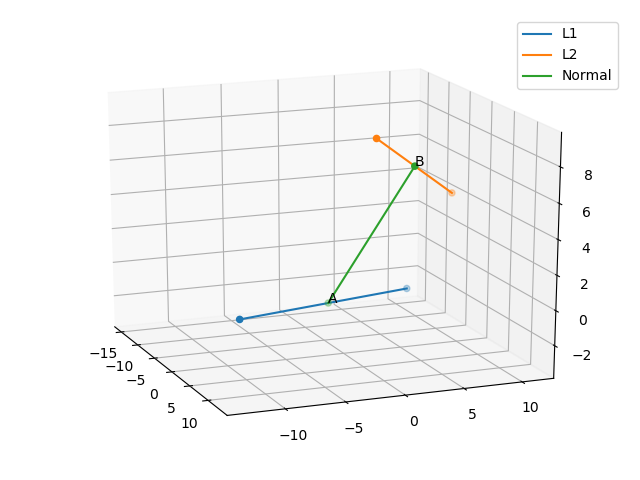
\includegraphics[width=\columnwidth]{chapters/12/11/2/15/figs/Figure_1.png}
\caption{}
\label{fig:chapters/12/11/2/15/}
\end{figure}


    \item Find the shortest distance between the lines whose vector equations are
    \begin{align}
\begin{split}
	\vec{x} &= \myvec{1\\2\\3} + \kappa_1\myvec{1\\-3\\2}
	\\
	\vec{x} &= \myvec{4\\5\\6} + \kappa_2\myvec{2\\3\\1}
\end{split}
        \label{eq:chapters/12/11/2/16/L2/svd}
    \end{align}
    \solution
		    In this case,
	    forming the matrix in \eqref{eq:chapters/12/11/2/16/lsq/rank},
    \begin{align*}
        \myvec{1&2&3\\-3&3&3\\2&1&3} \xleftrightarrow[]{R_2\leftarrow R_2+3R_1} \myvec{1&2&3\\0&9&12\\2&1&3} \\
                \xleftrightarrow[]{R_3\leftarrow R_3-2R_1} \myvec{1&2&3\\0&9&12\\0&-3&-3} %\\
                \xleftrightarrow[]{R_3\leftarrow 3R_3+R_2} \myvec{1&2&3\\0&9&12\\0&0&3}
                \label{eq:chapters/12/11/2/16/rank-aug}
    \end{align*}
    Clearly, the rank of this matrix is 3, and therefore, the lines are skew.
%
        From \eqref{eq:chapters/12/11/2/16/lsq/vec-eqn},
    \begin{align*}
        \augvec{2}{1}{14&-5&0\\-5&14&18} \xleftrightarrow[]{R_1\leftarrow R_1+R_2} \augvec{2}{1}{9&9&18\\-5&14&18} \\
                 \xleftrightarrow[]{R_1\leftarrow\frac{R_1}{9}} \augvec{2}{1}{1&1&2\\-5&14&18} 
                 \xleftrightarrow[]{R_2\leftarrow R_2+5R_1} \augvec{2}{1}{1&1&2\\0&19&28} \\
                 \xleftrightarrow[]{R_1\leftarrow19R_1-R_2} \augvec{2}{1}{19&0&10\\0&19&28} 
                 \xleftrightarrow[]{\substack{R_1\leftarrow\frac{R_1}{19}\\R_2\leftarrow\frac{R_2}{9}}}
                    \augvec{2}{1}{1&0&\frac{10}{19}\\0&1&\frac{28}{19}} \\
                    \implies \bm{\kappa} = \frac{1}{19}\myvec{10\\28}
    \end{align*}
        Substituting the above in \eqref{eq:chapters/12/11/2/16/L2/svd},
    \begin{align}
        \vec{x}_1 = \frac{1}{19}\myvec{29\\8\\77},\, \vec{x}_2 = \frac{1}{19}\myvec{20\\11\\86}.
    \end{align}
    Thus, the required distance is
    \begin{align}
        \norm{\vec{x}_2-\vec{x}_1} = \frac{3}{\sqrt{19}}
    \end{align}
See \figref{fig:chapters/12/11/2/16/skew}.
    \begin{figure}[!ht]
        \centering
        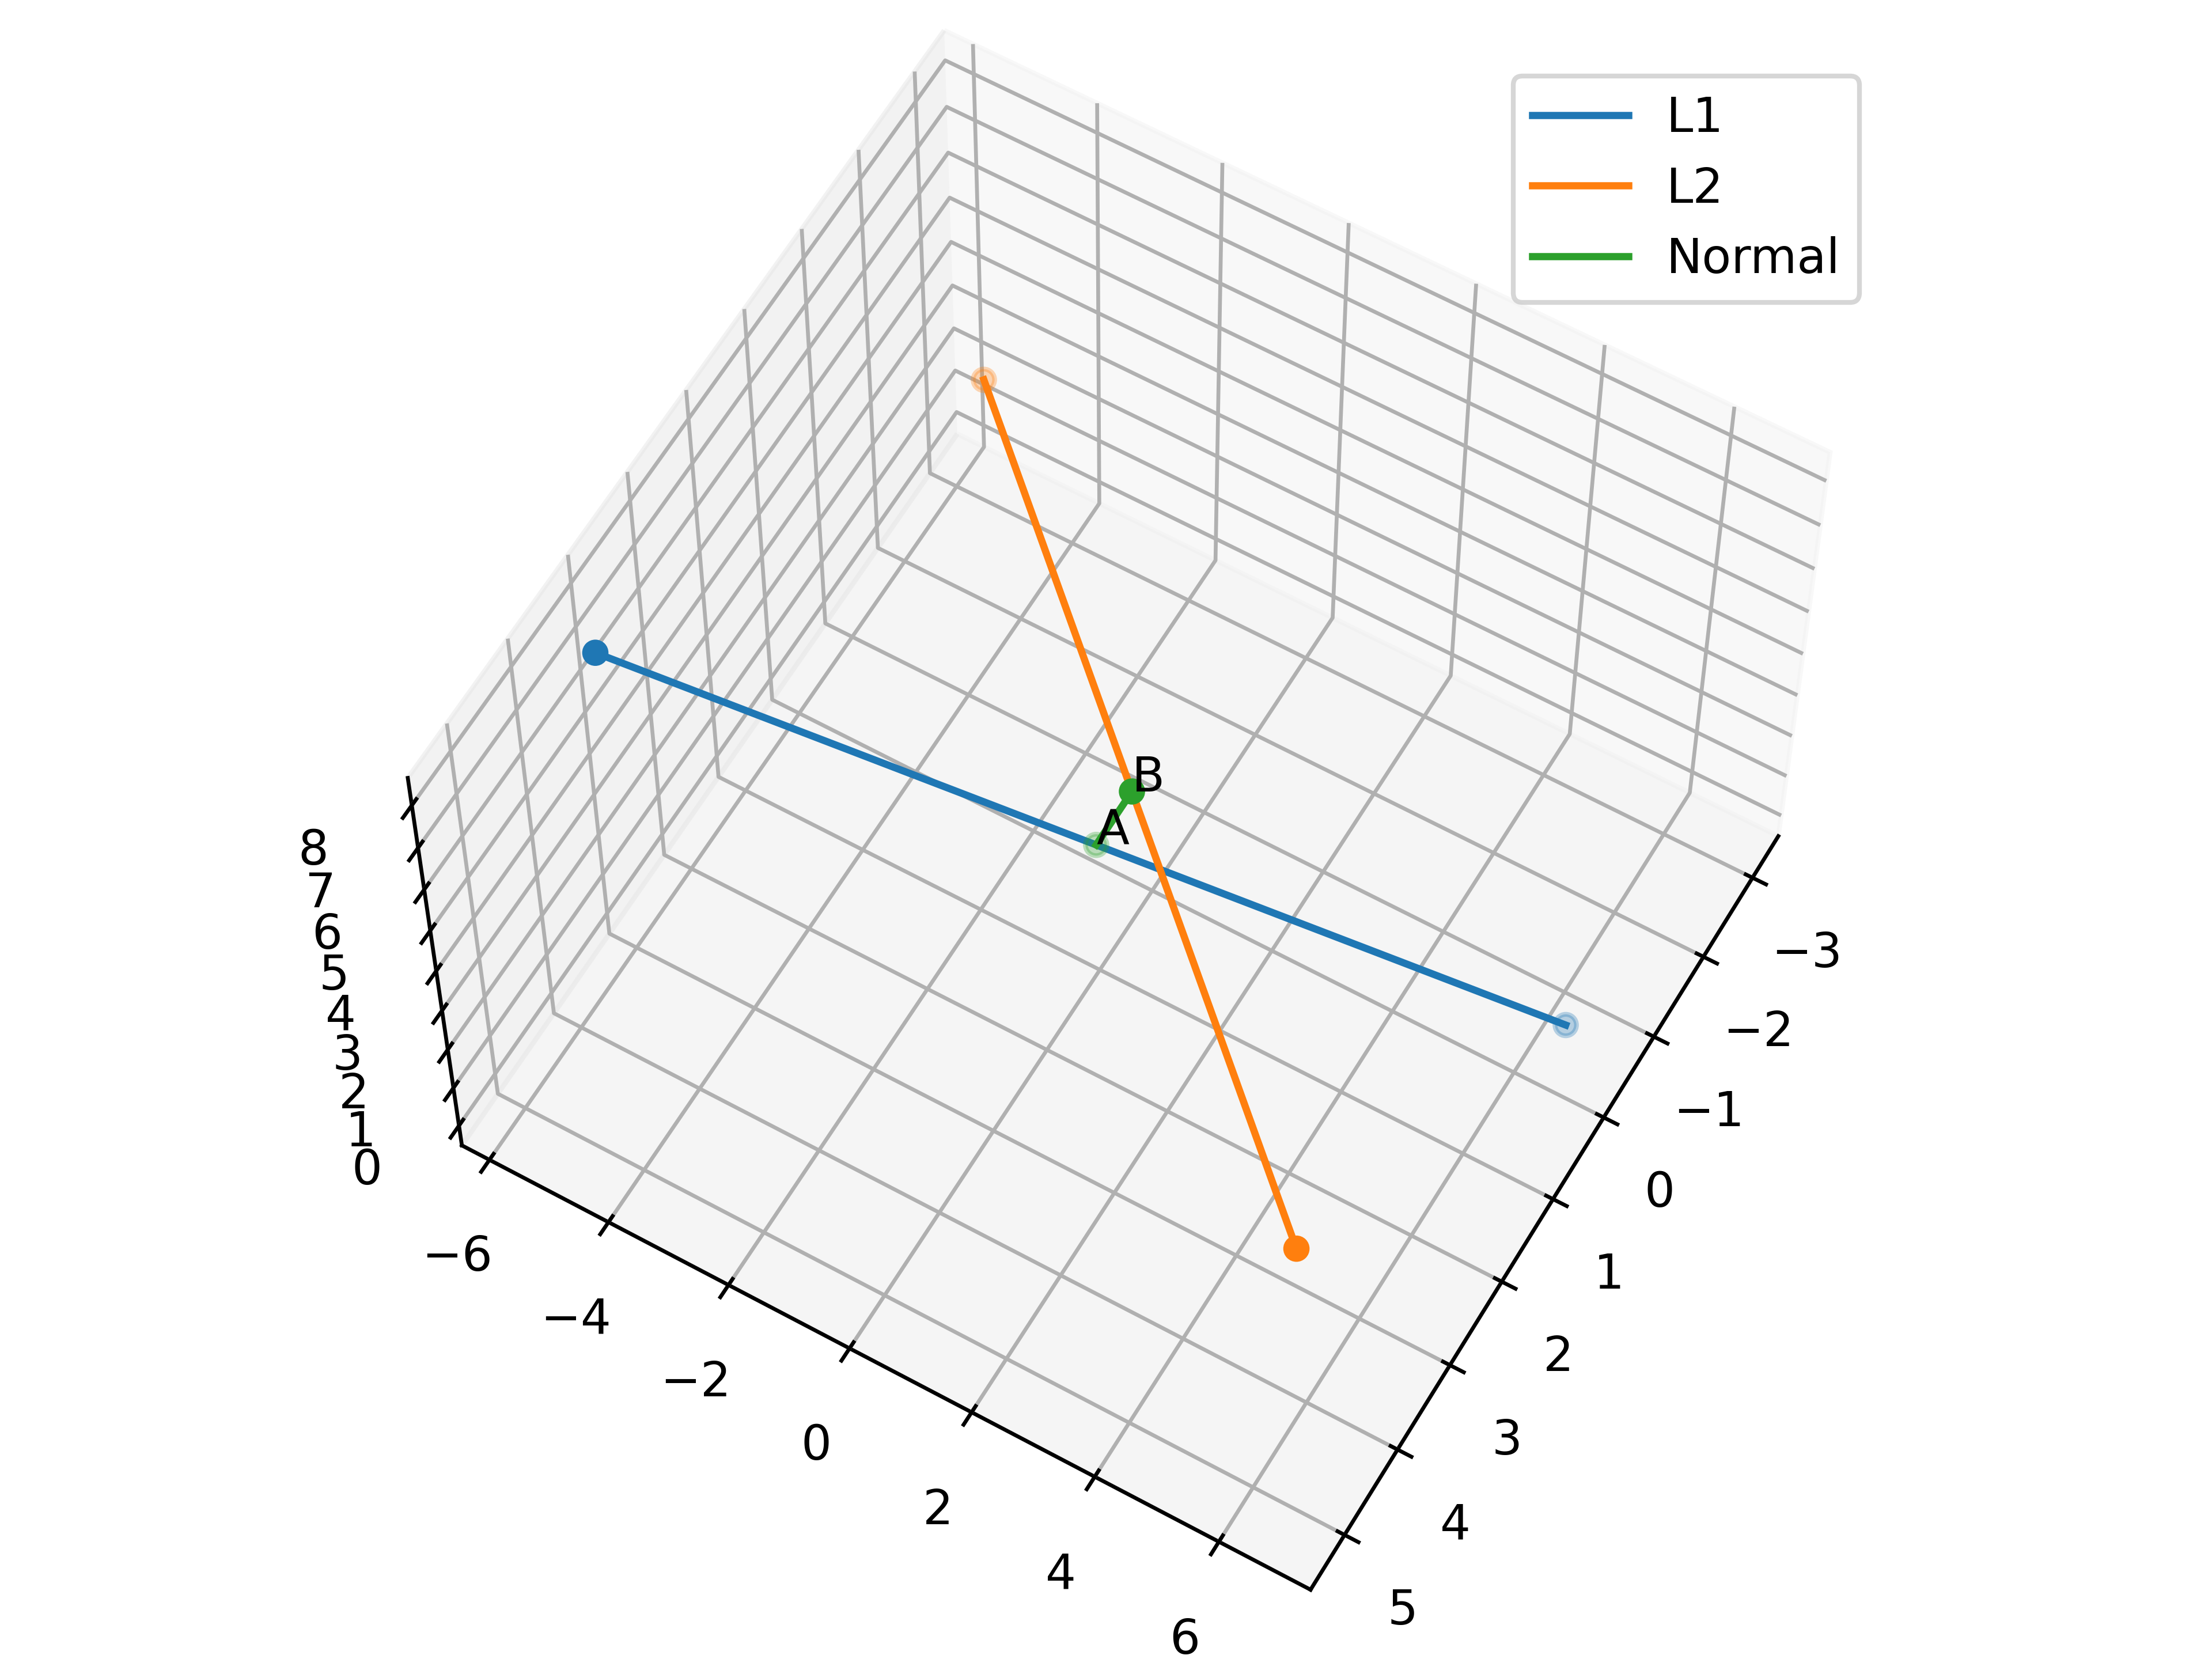
\includegraphics[width=\columnwidth]{chapters/12/11/2/16/lsq/figs/skew.png}
        \caption{}
        \label{fig:chapters/12/11/2/16/skew}
    \end{figure}

\item Find the shortest distance between the lines $l_1$ and $l_2$ whose vector equations are 
\begin{align}
	\overrightarrow{r} &= \hat{i}+\hat{j}+\kappa(2\hat{i}-\hat{j}+\hat{k}) \text{ and}
	\\
	\overrightarrow{r} &= 2\hat{i}+\hat{j}-\hat{k}+\mu(3\hat{i}-5\hat{j}+2\hat{k}).
\end{align}
    \solution
				The given lines can be written  in vector form  as
\begin{align}
\begin{split}
	\vec{x} &= \myvec{1\\1\\0} + \kappa_1\myvec{2\\-1\\1},
	\\
	\vec{x} &= \myvec{2\\1\\-1} + \kappa_2\myvec{3\\-5\\2}
\end{split}
\label{eq:chapters/12/11/2/e11/lines}
\\
\begin{split}
	\vec{M} &= \myvec{2&3\\-1&-5\\1&2},
\vec{B} - \vec{A} = \myvec{1\\0\\-1}
\end{split}
\label{eq:chapters/12/11/2/e11/params}
\end{align}
%
Substituting the above in \eqref{eq:chapters/12/11/2/16/lsq/rank},
\begin{align}
\myvec{2&3&1\\-1&-5&0\\1&2&-1}
\xleftrightarrow[R_3 \leftarrow R_3 - \frac{1}{2}R_1]{R_2 \leftarrow R_2 + \frac{1}{2}R_1}
	\myvec{2&3&1\\[1ex]0&-\frac{7}{2}&\frac{1}{2}\\[1ex]0&\frac{1}{2}&-\frac{3}{2}}\\
\xleftrightarrow{R_3 \leftarrow R_3 + 7R_2}
	\myvec{2&3&1\\[1ex]0&-\frac{7}{2}&\frac{1}{2}\\[1ex]0&0&-10}
\end{align}
The rank of the matrix is 3. So the given lines are skew.
        From \eqref{eq:chapters/12/11/2/16/lsq/vec-eqn},
\begin{align}
\myvec{2&-1&1\\3&-5&2} \myvec{2&3\\-1&-5\\1&2}\bm{\kappa} &= \myvec{2&-1&1\\3&-5&2} \myvec{1\\0\\-1}\\
\implies \myvec{6&13\\13&38}\bm{\kappa} &= \myvec{1\\1}
\label{eq:chapters/12/11/2/e11/3}
\end{align}
The augmented matrix of the above equation \eqref{eq:chapters/12/11/2/e11/3} is given by,
\begin{align}
\myvec{6&13&\vrule&1\\13&38&\vrule&1}
\xleftrightarrow{R_2 \leftarrow R_2 - \frac{13}{6}R_1}
\myvec{6&13&\vrule&1 \\ 0&\frac{59}{6}&\vrule&-\frac{7}{6}}\\
\xleftrightarrow{R_1 \leftarrow R_1 - \frac{78}{59}R_2}
\myvec{6&0&\vrule&\frac{150}{59} \\ 0&\frac{59}{6}&\vrule&-\frac{7}{6}}
\end{align}
yielding
\begin{align}
	\myvec{\kappa_1\\-\kappa_2} &= \myvec{\frac{25}{59}\\[1ex]-\frac{7}{59}}
	\label{eq:chapters/12/11/2/e11/}
\end{align}
Substituting in \eqref{eq:chapters/12/11/2/e11/lines},
\begin{align}
\vec{x}_1 
= \frac{1}{59}\myvec{109\\34\\25},\,
\vec{x}_2 
= \frac{1}{59}\myvec{139\\24\\-45}.
\end{align}
The minimum distance between the lines is given by,
\begin{align}
\norm{\vec{x}_2-\vec{x}_1} &= \norm{\frac{1}{59}\myvec{30\\-10\\-70}}
= \frac{10}{\sqrt{59}}
\end{align}
See Fig. 
	\ref{fig:chapters/12/11/2/e11/}.
\begin{figure}[!ht]
\centering
\includegraphics[width=\columnwidth]{chapters/12/11/2/e11/lsq/figs/skew.png}
\caption{}
	\label{fig:chapters/12/11/2/e11/}
\end{figure}

		%\iffalse
\documentclass[journal,12pt,twocolumn]{IEEEtran}
\usepackage{romannum}
\usepackage{float}
\usepackage{setspace}
\usepackage{gensymb}
\singlespacing
\usepackage[cmex10]{amsmath}
\usepackage{amsthm}
\usepackage{mathrsfs}
\usepackage{txfonts}
\usepackage{stfloats}
\usepackage{bm}
\usepackage{cite}
\usepackage{cases}
\usepackage{subfig}
\usepackage{longtable}
\usepackage{multirow}
\usepackage{enumitem}
\usepackage{mathtools}
\usepackage{steinmetz}
\usepackage{tikz}
\usepackage{circuitikz}
\usepackage{verbatim}
\usepackage{tfrupee}
\usepackage[breaklinks=true]{hyperref}
\usepackage{tkz-euclide}
\usetikzlibrary{calc,math}
\usepackage{listings}
    \usepackage{color}                                            %%
    \usepackage{array}                                            %%
    \usepackage{longtable}                                        %%
    \usepackage{calc}                                             %%
    \usepackage{multirow}                                         %%
    \usepackage{hhline}                                           %%
    \usepackage{ifthen}                                           %%
  %optionally (for landscape tables embedded in another document): %%
    \usepackage{lscape}     
\usepackage{multicol}
\usepackage{chngcntr}
\DeclareMathOperator*{\Res}{Res}
\renewcommand\thesection{\arabic{section}}
\renewcommand\thesubsection{\thesection.\arabic{subsection}}
\renewcommand\thesubsubsection{\thesubsection.\arabic{subsubsection}}

\renewcommand\thesectiondis{\arabic{section}}
\renewcommand\thesubsectiondis{\thesectiondis.\arabic{subsection}}
\renewcommand\thesubsubsectiondis{\thesubsectiondis.\arabic{subsubsection}}

% correct bad hyphenation here
\hyphenation{op-tical net-works semi-conduc-tor}
\def\inputGnumericTable{}                                 %%

\lstset{
frame=single, 
breaklines=true,
columns=fullflexible
}

\begin{document}


\newtheorem{theorem}{Theorem}[section]
\newtheorem{problem}{Problem}
\newtheorem{proposition}{Proposition}[section]
\newtheorem{lemma}{Lemma}[section]
\newtheorem{corollary}[theorem]{Corollary}
\newtheorem{example}{Example}[section]
\newtheorem{definition}[problem]{Definition}
\newcommand{\BEQA}{\begin{eqnarray}}
\newcommand{\EEQA}{\end{eqnarray}}
\newcommand{\define}{\stackrel{\triangle}{=}}

\bibliographystyle{IEEEtran}
\providecommand{\mbf}{\mathbf}
\providecommand{\pr}[1]{\ensuremath{\Pr\left(#1\right)}}
\providecommand{\qfunc}[1]{\ensuremath{Q\left(#1\right)}}
\providecommand{\sbrak}[1]{\ensuremath{{}\left[#1\right]}}
\providecommand{\lsbrak}[1]{\ensuremath{{}\left[#1\right.}}
\providecommand{\rsbrak}[1]{\ensuremath{{}\left.#1\right]}}
\providecommand{\brak}[1]{\ensuremath{\left(#1\right)}}
\providecommand{\lbrak}[1]{\ensuremath{\left(#1\right.}}
\providecommand{\rbrak}[1]{\ensuremath{\left.#1\right)}}
\providecommand{\cbrak}[1]{\ensuremath{\left\{#1\right\}}}
\providecommand{\lcbrak}[1]{\ensuremath{\left\{#1\right.}}
\providecommand{\rcbrak}[1]{\ensuremath{\left.#1\right\}}}
\theoremstyle{remark}
\newtheorem{rem}{Remark}
\newcommand{\sgn}{\mathop{\mathrm{sgn}}}
\providecommand{\abs}[1]{\left\vert#1\right\vert}
\providecommand{\res}[1]{\Res\displaylimits_{#1}} 
\providecommand{\norm}[1]{\left\lVert#1\right\rVert}
\providecommand{\mtx}[1]{\mathbf{#1}}
\providecommand{\mean}[1]{E\left[ #1 \right]}
\providecommand{\fourier}{\overset{\mathcal{F}}{ \rightleftharpoons}}
\providecommand{\system}{\overset{\mathcal{H}}{ \longleftrightarrow}}
\newcommand{\solution}{\noindent \textbf{Solution: }}
\newcommand{\cosec}{\,\text{cosec}\,}
\providecommand{\dec}[2]{\ensuremath{\overset{#1}{\underset{#2}{\gtrless}}}}
\newcommand{\myvec}[1]{\ensuremath{\begin{pmatrix}#1\end{pmatrix}}}
\newcommand{\mydet}[1]{\ensuremath{\begin{vmatrix}#1\end{vmatrix}}}
\numberwithin{equation}{subsection}
\makeatletter
\@addtoreset{figure}{problem}
\makeatother

\let\StandardTheFigure\thefigure
\let\vec\mathbf
\renewcommand{\thefigure}{\theproblem}



\def\putbox#1#2#3{\makebox[0in][l]{\makebox[#1][l]{}\raisebox{\baselineskip}[0in][0in]{\raisebox{#2}[0in][0in]{#3}}}}
     \def\rightbox#1{\makebox[0in][r]{#1}}
     \def\centbox#1{\makebox[0in]{#1}}
     \def\topbox#1{\raisebox{-\baselineskip}[0in][0in]{#1}}
     \def\midbox#1{\raisebox{-0.5\baselineskip}[0in][0in]{#1}}

\vspace{3cm}


\title{Assignment 1}
\author{Jaswanth Chowdary Madala}





% make the title area
\maketitle

\newpage

%\tableofcontents

\bigskip

\renewcommand{\thefigure}{\theenumi}
\renewcommand{\thetable}{\theenumi}

\begin{enumerate}
\item Find the shortest distance between the lines $l_1$ and $l_2$ whose vector equations are ${\overrightarrow{r} = \hat{i}+\hat{j}+\lambda(2\hat{i}-\hat{j}+\hat{k})}$ and ${\overrightarrow{r} = 2\hat{i}+\hat{j}-\hat{k}+\mu(3\hat{i}-5\hat{j}+2\hat{k})}$

\textbf{Solution:} 
\fi
The shortest distance between the lines whose vector equations are
\begin{align}
L_1: \vec{x} = \vec{x_1} + \lambda_1\vec{m_1} \label{eq:chapters/12/11/2/311/svd/1} \\
L_2: \vec{x} = \vec{x_2} + \lambda_2\vec{m_2} \label{eq:chapters/12/11/2/311/svd/2}
\end{align}
is given by,
\begin{align}
d = \norm{\brak{\vec{U}\brak{\vec{\Sigma\Sigma}^{-1}}\vec{U}^\top-\vec{I}}\vec{x}}
\end{align}
with the parameter $\lambda$ given by
\begin{align}
\bm{\lambda} = \vec{V\Sigma}^{-1}\vec{U}^\top\vec{x} \label{eq:chapters/12/11/2/311/svd/lambda-sol}
\end{align}
where
\begin{align}
\vec{M} &\triangleq \myvec{\vec{m_1} & \vec{m_2}} \label{eq:chapters/12/11/2/311/svd/3}\\
\bm{\lambda} &\triangleq \myvec{\lambda_1\\-\lambda_2}\label{eq:chapters/12/11/2/311/svd/4} \\
\vec{x} &\triangleq \vec{x_2} - \vec{x_1} \label{eq:chapters/12/11/2/311/svd/5}
\end{align}

We use singular value decomposition of the matrix $\vec{M}$
\begin{align}
\vec{M} = \vec{U\Sigma V}^\top \label{eq:chapters/12/11/2/311/svd/6}
\end{align}
where $\vec{U}, \vec{V}$ are orthogonal and $\vec{\Sigma}$ is diagonal with nonnegative diagonal entries.

\begin{enumerate}
\item In this problem we have the lines $l_1$ and $l_2$ as
\begin{align}
\vec{x} &= \myvec{1\\1\\0} + \lambda_1\myvec{2\\-1\\1}\\
\vec{x} &= \myvec{2\\1\\-1} + \lambda_2\myvec{3\\-5\\2}
\end{align}

We first need to check whether the given lines are skew.
The lines \eqref{eq:chapters/12/11/2/311/svd/1}, \eqref{eq:chapters/12/11/2/311/svd/2} intersect if
\begin{align}
\vec{M}\bm{\lambda} &= \vec{x_2} - \vec{x_1}
\end{align}
Here we have,
\begin{align}
\vec{M} &= \myvec{2&3\\-1&-5\\1&2} \label{eq:chapters/12/11/2/311/svd/M}\\
\vec{x} = \vec{x_2} - \vec{x_1} &= \myvec{1\\0\\-1} \label{eq:chapters/12/11/2/311/svd/x}
\end{align}
We check whether the equation \eqref{eq:chapters/12/11/2/311/svd/7} has a solution
\begin{align}
\myvec{2&3\\-1&-5\\1&2}\bm{\lambda} = \myvec{1\\0\\-1}
\label{eq:chapters/12/11/2/311/svd/7}
\end{align}
the augmented matrix is given by,
\begin{align}
&\myvec{2&3&\vrule&1\\-1&-5&\vrule&0\\1&2&\vrule&-1}\\
\xleftrightarrow[R_3 \leftarrow R_3 - \frac{1}{2}R_1]{R_2 \leftarrow R_2 + \frac{1}{2}R_1}
&\myvec{2&3&\vrule&1\\&&\vrule\\0&-\frac{7}{2}&\vrule&\frac{1}{2}\\&&\vrule\\0&\frac{1}{2}&\vrule&-\frac{3}{2}}\\
\xleftrightarrow{R_3 \leftarrow R_3 + 7R_2}
&\myvec{2&3&\vrule&1\\&&\vrule\\0&-\frac{7}{2}&\vrule&\frac{1}{2}\\&&\vrule\\0&0&\vrule&-10}
\end{align}
The rank of the matrix is 3. So the given lines are skew.

\item From \eqref{eq:chapters/12/11/2/311/svd/M} we have
\begin{align}
\vec{M}^\top\vec{M} &= \myvec{2&-1&1\\3&-5&2}\myvec{2&3\\-1&-5\\1&2} \\ 
&= \myvec{6&13\\13&38} \label{eq:chapters/12/11/2/311/svd/MtM}
\end{align}
\begin{align}
\vec{MM}^\top &= \myvec{2&3\\-1&-5\\1&2}\myvec{2&-1&1\\3&-5&2}\\
&= \myvec{13&-17&8\\-17&26&-11\\8&-11&5} \label{eq:chapters/12/11/2/311/svd/MMt}
\end{align}
We perform the eigen decompositions for the matrics \eqref{eq:chapters/12/11/2/311/svd/MMt}, \eqref{eq:chapters/12/11/2/311/svd/MtM} and write them in the form
\begin{align}
    \vec{MM}^\top &= \vec{P_1D_1P_1}^\top \label{eq:chapters/12/11/2/311/svd/decomp-1} \\
    \vec{M}^\top\vec{M} &= \vec{P_2D_2P_2}^\top \label{eq:chapters/12/11/2/311/svd/decomp-2}
\end{align}
The characteristic polynomial of the matrix $\vec{MM}^\top$ is given by,
\begin{align}
\text{char}\brak{\vec{MM}^\top} &= \mydet{13-x&-17&8\\-17&26-x&-11\\8&-11&5-x} \\
&= -x^3 + 44x^2-59x
%\label{eq:chapters/12/11/2/311/svd/char-1}
\end{align}
Thus, the eigenvalues are given by
\begin{align}
\lambda_1 = 22+5\sqrt{17},\ \lambda_2 = 22-5\sqrt{17},\ \lambda_3 = 0
\end{align}
From the augmented matrix formed from the eigen value - eigen vector equation we get, the normalized eigen vectors as
\begin{align}
    \vec{p_1} &= \frac{\sqrt{5}}{\sqrt{68-6\sqrt{17}}} \myvec{\frac{12-\sqrt{17}}{5}\\\frac{1-3\sqrt{17}}{5}\\1}\\
    \vec{p_2} &= \frac{\sqrt{5}}{\sqrt{68+6\sqrt{17}}} \myvec{\frac{12+\sqrt{17}}{5}\\\frac{1+3\sqrt{17}}{5}\\1}\\
    \vec{p_3} &= \frac{1}{\sqrt{59}}\myvec{-3\\1\\7}
\end{align}
where $\vec{p_1},\vec{p_2},\vec{p_3}$ corresponds to the  eigen values $\lambda_1, \lambda_2, \lambda_3$ respectively. Using \eqref{eq:chapters/12/11/2/311/svd/decomp-1}, we get
\begin{align}
    \vec{P_1} &= \myvec{\frac{12-\sqrt{17}}{\sqrt{5}\sqrt{68-6\sqrt{17}}} & \frac{12+\sqrt{17}}{\sqrt{5}\sqrt{68+6\sqrt{17}}} & -\frac{3}{\sqrt{59}}\\
    \frac{1-3\sqrt{17}}{\sqrt{5}\sqrt{68-6\sqrt{17}}}&\frac{1+3\sqrt{17}}{\sqrt{5}\sqrt{68+6\sqrt{17}}} & \frac{1}{\sqrt{59}}\\
\frac{\sqrt{5}}{\sqrt{68-6\sqrt{17}}}&\frac{\sqrt{5}}{\sqrt{68+6\sqrt{17}}} & \frac{7}{\sqrt{59}} }
    \label{eq:chapters/12/11/2/311/svd/eig-params-1(a)}
\end{align}
\begin{align}
    \vec{D_1} &= \myvec{22+5\sqrt{17}&0&0\\0&22-5\sqrt{17}&0\\0&0&0}
    \label{eq:chapters/12/11/2/311/svd/eig-params-1(b)}
\end{align}

For $\vec{M}^\top\vec{M}$, the characteristic polynomial is
\begin{align}
    \text{char}\brak{\vec{M}^\top\vec{M}} &= \mydet{6-x&13\\13&38-x} \\&= x^2-44x+59
    \label{eq:chapters/12/11/2/311/svd/char-1}
\end{align}
Thus, the eigenvalues are given by
\begin{align}
    \lambda_1 = 22+5\sqrt{17},\ \lambda_2 = 22-5\sqrt{17}
\end{align}
From the augmented matrix formed from the eigen value - eigen vector equation we get, the normalized eigen vectors as
\begin{align}
\vec{p_1} &= \frac{13}{\sqrt{850-160\sqrt{17}}}\myvec{\frac{-16+5\sqrt{17}}{13}\\1}\\
\vec{p_2} &= \frac{13}{\sqrt{850+160\sqrt{17}}} \myvec{\frac{-16-5\sqrt{17}}{13}\\1}
\end{align}
where $\vec{p_1},\vec{p_2}$ corresponds to the  eigen values $\lambda_1, \lambda_2$ respectively. Using \eqref{eq:chapters/12/11/2/311/svd/decomp-2}, we get
\begin{align}
    \vec{P_2} &= \myvec{\frac{-16-5\sqrt{17}}{\sqrt{850+160\sqrt{17}}}&\frac{13}{\sqrt{850-160\sqrt{17}}}\\\frac{13}{\sqrt{850+160\sqrt{17}}}&\frac{-16+5\sqrt{17}}{\sqrt{850-160\sqrt{17}}}}
     \label{eq:chapters/12/11/2/311/svd/eig-params-2(a)}\\ 
    \vec{D_2} &= \myvec{22-5\sqrt{17}&0\\0&22+5\sqrt{17}}
    \label{eq:chapters/12/11/2/311/svd/eig-params-2(b)}
\end{align}
Therefore, from \eqref{eq:chapters/12/11/2/311/svd/6} we have
\begin{align}
    \vec{U} &= \vec{P_1} \\ 
    \vec{V} &= \vec{P_2} \\
    \vec{\Sigma} &= \myvec{\sqrt{22+5\sqrt{17}}&0\\0&\sqrt{22-5\sqrt{17}}\\0&0}
    \label{eq:chapters/12/11/2/311/svd/svd-params}
\end{align}
and substituting into \eqref{eq:chapters/12/11/2/311/svd/lambda-sol}, we get
\begin{align}
    \bm{\lambda} =  \myvec{\frac{25}{59}\\\\-\frac{7}{59}}
\end{align}
The minimum distance between the lines is given by,
\begin{align}
\norm{\vec{B}-\vec{A}} &= \norm{\frac{1}{59}\myvec{30\\-10\\-70}}\\
&= \frac{\sqrt{30^2+10^2+70^2}}{59}\\
&= \frac{10}{\sqrt{59}}
\end{align}
The shortest distance between the given lines is $\frac{10}{\sqrt{59}}$ units.
See Fig. 
	\ref{fig:chapters/12/11/2/e11/svd/}.
\begin{figure}[!ht]
\centering
\includegraphics[width=\columnwidth]{./chapters/12/11/2/e11/svd/figs/skew.png}
\caption{$AB$ is the required shortest distance.}
	\label{fig:chapters/12/11/2/e11/svd/}
\end{figure}
\end{enumerate} 

\item Find the shortest distance between the lines given by 
\begin{align}
	\overrightarrow{r}&=(8+3\kappa\hat{i}-(9+16\kappa)\hat{j}+(10+7\kappa)\hat{k} \text{ and} 
	\\
	\overrightarrow{r}&=15\hat{i}+29\hat{j}+5\hat{k}+\mu(3\hat{i}+8\hat{j}-5\hat{k}).
\end{align}
\item Find the shortest distance between the lines
\begin{align}
	\overrightarrow{r}&=(\hat{i}+2\hat{j}+\hat{k})+\kappa(\hat{i}-\hat{j}+\hat{k}) \text{ and} 
	\\
	\overrightarrow{r}&=2\hat{i}-\hat{j}-\hat{k}+\mu(2\hat{i}+\hat{j}+2\hat{k})
\end{align}
\item Find the matrix $\vec{X}$ so that $\vec{X}\myvec{1&2&3\\ 4&5&6}$= $\myvec{-7&-8&-9\\ 2&4&6}$.
\end{enumerate}
